\documentclass[conference]{IEEEtran}
\IEEEoverridecommandlockouts
\usepackage{cite}
\usepackage{amsmath,amssymb,amsfonts}
\usepackage{algorithmic}
\usepackage{graphicx}
\usepackage{textcomp}
\usepackage{xcolor}
\usepackage[brazilian]{babel}
\usepackage[utf8]{inputenc}
\usepackage[T1]{fontenc}
\def\BibTeX{{\rm B\kern-.05em{\sc i\kern-.025em b}\kern-.08em
    T\kern-.1667em\lower.7ex\hbox{E}\kern-.125emX}}
\begin{document}

\title{Perceptron de Multiplas camadas para Diagnóstico de Câncer de Mama}

\author{\IEEEauthorblockN{1\textsuperscript{o} Anara Olimpio}
    \IEEEauthorblockA{
        \textit{anaraolimpio@ig.com.br}
    }
    \and
    \IEEEauthorblockN{2\textsuperscript{o} Bruno Lopes}
    \IEEEauthorblockA{
        \textit{bruno.lopes.ti@icloud.com}
    }
    \and
}
\maketitle

\begin{abstract}
O câncer de mama é considerado o segundo tipo de câncer mais recorrente em mulheres, perdendo somente para o câncer de pele. De acordo com dados do Instituto Nacional do Câncer (INCA), em 2014, ocorreram mais de 57 mil casos de câncer de mama no Brasil em mulheres e, embora em quantidades bem pequenas, em homens. Diante do número alto de incidências, principalmente em mulheres, existe uma grande necessidade de pesquisa sobre o assunto. Este trabalho será baseado numa proposta de utilização de rede neural artificial para obter informações mais rápidas sobre o diagnóstico do câncer de mama utilizando como base para estudo e desenvolvimento do trabalho o conjunto de dados Breast Cancer Wisconsin. Este conjunto de dados de câncer de mama foi obtido do Hospital Universidade de Wisconsin, Madison, do Dr. William H. Wolberg. Os dados foram coletados, periodicamente, entre 1989 e 1991 com a ajuda do doutor Wolberg ao relatar seus casos clínicos o que possibilitou coletar as medidas dos tumores de mama. Os dados refletem uma ordem cronológico da coleta de dados e é um conjunto de dados de classificação. Há duas classes determinadas: benignas e malignas. Este conjunto de dados possui 699 registros e dimensão de 9 e baseado nessas informações pretendemos criar um padrão de comportamento que seja ágil em predizer se o tumor é maligno ou benigno.

\end{abstract}

\begin{IEEEkeywords}
Perceptron. Artificial Neural Network. Breast Cancer Wisconsin
\end{IEEEkeywords}

\section{INTRODUÇÃO}

\section{Referencial Teórico}
	%Problema, base conceitual para a solucao %
	
	Nosso objetivo é utilizar a base de dados Breast Cancer Wisconsin \cite{b8} fornecida pelo Hospital Universidade de Wisconsin para treinar uma Rede Neural Artificial(RNA). Esses elementos serão utilizados pela nossa RNA, afim aprender a classificar quais tipos de tumores são malignos e quais são benignos. 
	
	Redes neurais artificiais são modelos inspirados na arquitetura neural do cérebro e foi desenvolvido para tentar modelar a capacidade de aprendizagem de sistemas neurais biológicos \cite{b4}. Uma arquitetura típica de RNA conhecida como Perceptron de Multicamadas (MLP) contém uma série de camadas, compostas de neurônios e suas conexões. Um neurônio artificial tem a capacidade de calcular a soma ponderada de suas entradas e, em seguida, aplica uma função de ativação para obter um sinal que será transmitido para o próximo neurônio.
	
	\subsection{Perceptron Simples}
	O Modelo Perceptron foi desenvolvido nas décadas de 1950 e 1960 pelo cientista Frank Rosenblatt \cite{b9}, inspirado em trabalhos anteriores de Warren McCulloch e Walter Pitts. Hoje, é mais comum usar outros modelos de neurônios artificiais, mas o Perceptron permite uma compreensão clara de como funciona uma rede neural em termos matemáticos.
	
	
    Aprendizagem ou treinamento de RNA é equivalente a encontrar os valores de todos os pesos de tal forma que a saída desejada é gerada para correspondente entrada, pode ser visto como a minimização da função de erro computada pela diferença entre a saída da rede e o desejado na saída de um conjunto de observações de treinamento \cite{b6}.
	
	Um Perceptron é um modelo matemático que recebe várias entradas, x1, x2, … xn e produz uma única saída binária, forme monstra na Figura 1.
	
	\begin{figure}[htbp]
	\centerline{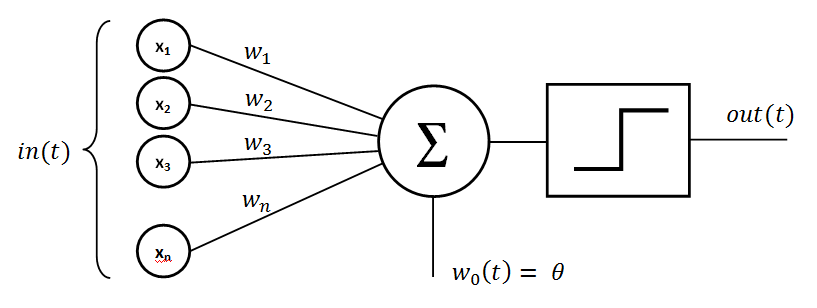
\includegraphics[scale=1]{Perceptron.png}}
	\caption{Perceptron simples}
	\label{fig}
	\end{figure}
	
	No exemplo mostrado, o Perceptron possui n entradas: x1, x2, … xn. Rosenblatt propôs uma regra simples para calcular a saída. Ele introduziu pesos, w1, w2, …, números reais expressando a importância das respectivas entradas para a saída. A saída do neurônio, 0 ou 1, é determinada pela soma ponderada, menor ou maior do que algum valor limiar (threshold). Assim como os pesos, o threshold é um número real que é um parâmetro do neurônio. Em termos algébricos temos:
	
	\begin{figure}[htbp]
	\centerline{
\includegraphics[scale=0.8]{Perceptron-threshold.png}}
	\caption{Soma Ponderada com threshold}
	\label{fig}
	\end{figure}

    O Perceptron é um classificador linear (binário). Além disso, é usado na aprendizagem supervisionada e pode ser usado para classificar os dados de entrada fornecidos.
    
    Um único Perceptron consegue resolver somente funções linearmente separáveis,  mas como nosso modelo de dados tem caracteristicas não linear, com podemos ver na Figura 3, o Perceptron não consegue gerar um hiperplano para separar os dados. Por isso buscamos uma variante do modelo de Perceptron simples, o Perceptron de multicamadas.
    
    \begin{figure}[htbp]
	\centerline{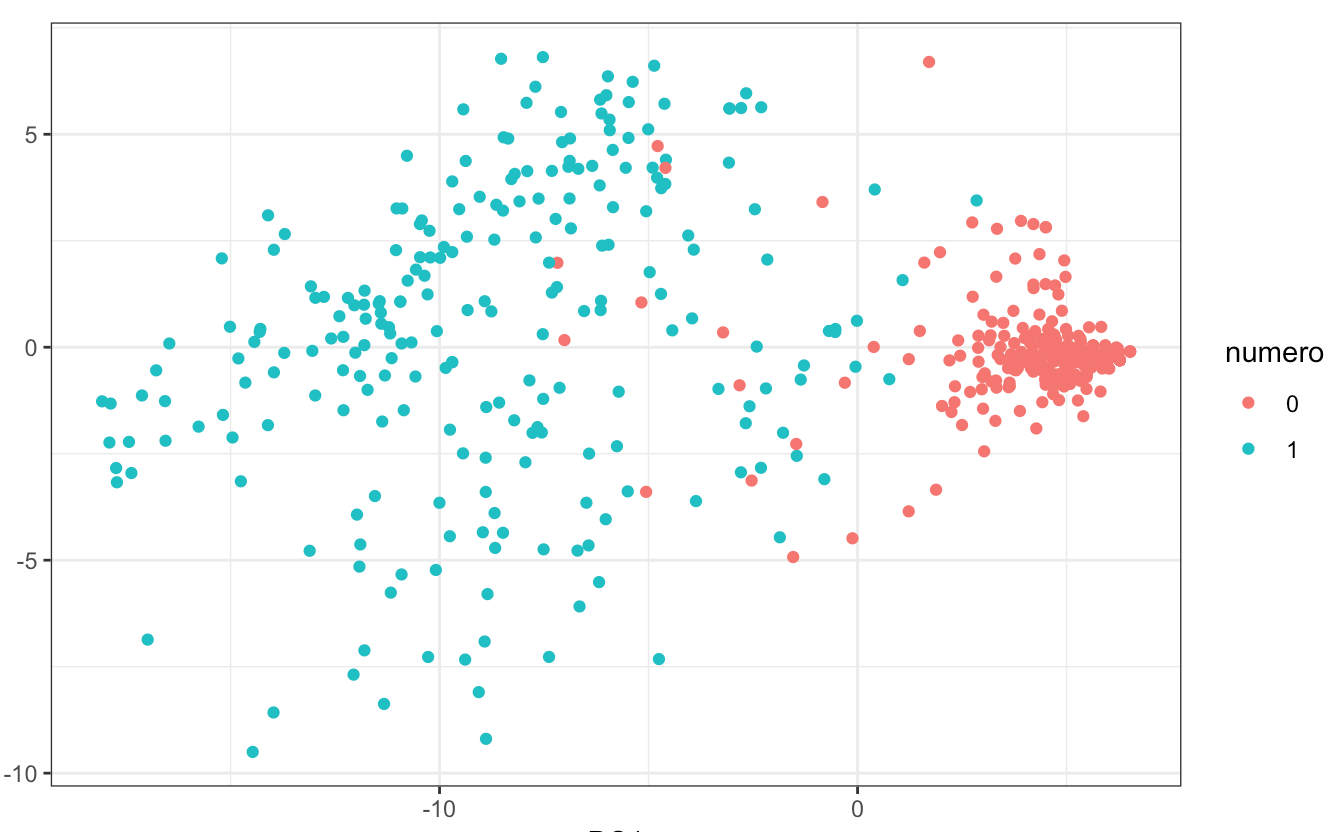
\includegraphics[scale=0.3]{dados-cancer.png}}
	\caption{Amostra dos dados (0 = benigno, 1 = maligno)}
	\label{fig}
	\end{figure}
    
    \subsection{Perceptron de multicamada}
    Um Perceptron de multicamadas é uma variante do modelo Perceptron original proposto por Rosenblatt na década de 1950 \cite{b9}. Tem uma ou mais camadas escondidas entre suas camadas de entrada e saída, os neurônios são organizados em camadas, as conexões são sempre direcionadas de camadas inferiores para camadas, os neurônios na mesma camada não estão interligados, conforme ilustrado na Figura 4.
    
    \begin{figure}[htbp]
	\centerline{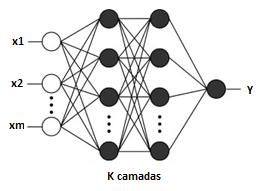
\includegraphics[scale=0.9]{Perceptron-Multicamadas.png}}
	\caption{Perceptron Multicamadas}
	\label{fig}
	\end{figure}
    
    A definição da arquitetura em redes MLP é um ponto muito relevante, a falta de conexões pode tornar a rede incapaz de resolver o problema de parâmetros ajustáveis, enquanto um excesso de conexões pode causar um ajuste excessivo dos dados de treinamento \cite{b7}.

    \subsection{Base de Dados}

O banco de dados utilizado nesse experimento foi obtido da Universidade de Wisconsin Hospitals \cite{b10} \cite{b11}. Os atributos 2 a 10 foram usados para representar instâncias. Cada instância tem uma das duas classes possíveis: benigna ou maligna.
    
    As amostras chegam periodicamente enquanto o Dr. Wolberg relata seus casos clínicos.
   O banco de dados, portanto, reflete esse agrupamento cronológico dos dados.
   Esta informação de agrupamento aparece imediatamente abaixo, tendo sido removida
   dos dados em si:

\begin{description}
     \item Grupo 1: 367 instâncias (janeiro de 1989)
     \item Grupo 2: 70 instâncias (outubro de 1989)
     \item Grupo 3: 31 instâncias (fevereiro de 1990)
     \item Grupo 4: 17 instâncias (abril de 1990)
     \item Grupo 5: 48 instâncias (agosto de 1990)
     \item Grupo 6: 49 instâncias (janeiro de 1991)
     \item Grupo 7: 31 instâncias (junho de 1991)
     \item Grupo 8: 86 instâncias (novembro de 1991)
\end{description}
    No total são 699 (a partir da base de dados doada em 15 de julho de 1992) \cite{b10} \cite{b11}. Observe que os resultados resumidos acima em uso, referem-se a um conjunto de dados
    de tamanho 369, enquanto o Grupo 1 tem apenas 367 instâncias. Isso é porque originalmente continha 369 instâncias; 2 foram removidos. 
   
   Temos no total 10 atributos mais a classe, conforme abaixo:
    \begin{enumerate}
    
   \item  Sample code number
   \item  Clump Thickness
   \item  Uniformity of Cell Size
   \item  Uniformity of Cell Shape
   \item  Marginal Adhesion
   \item  Single Epithelial Cell Size
   \item  Bare Nuclei
   \item  Bland Chromatin
   \item  Normal Nucleoli
   \item  Mitoses
   \item  Classe: (2 for benign, 4 for malignant)
    \end{enumerate}
    
    Existem 16 registros com dados inválidos dentro do arquivo, eles foram retirados para que o resultado final não fosse prejudicado, pois os mesmos vieram com o sinal "?" no campo X1.3. Dessa forma temos a seguinte distribuição para treinamento: Benigno: 458 (65.5\%) Maligno: 241 (34.5\%)

	
	
\section{Avaliação de Desenpenho}
    % Metodologia, experimentos e resultados, analise dos resultados(porques) %
    
        \begin{figure}[htbp]
	\centerline{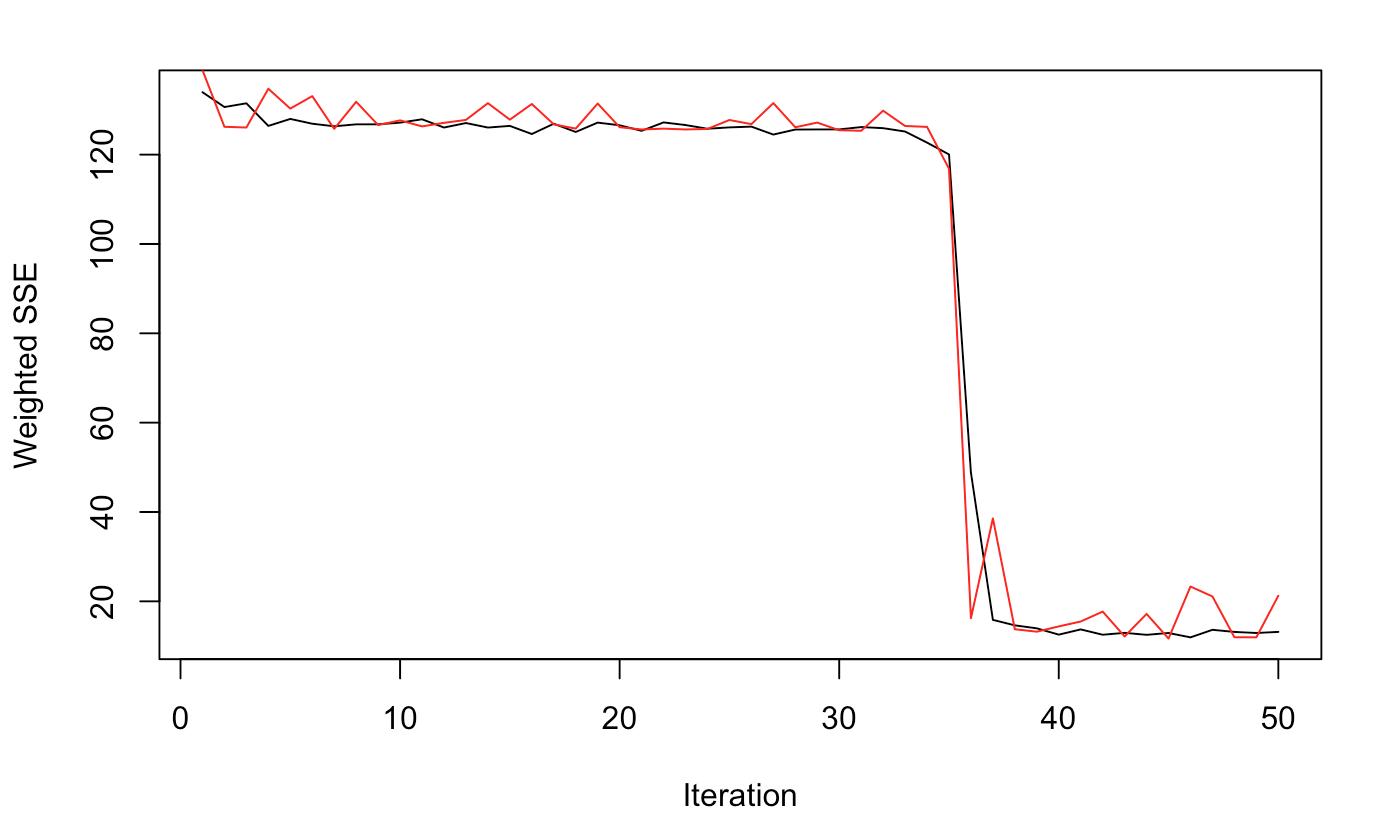
\includegraphics[scale=0.4]{imagens/9,8,8,5,3-50.png}}
	\caption{Função de Custo 50 iterações}
	
	\centerline{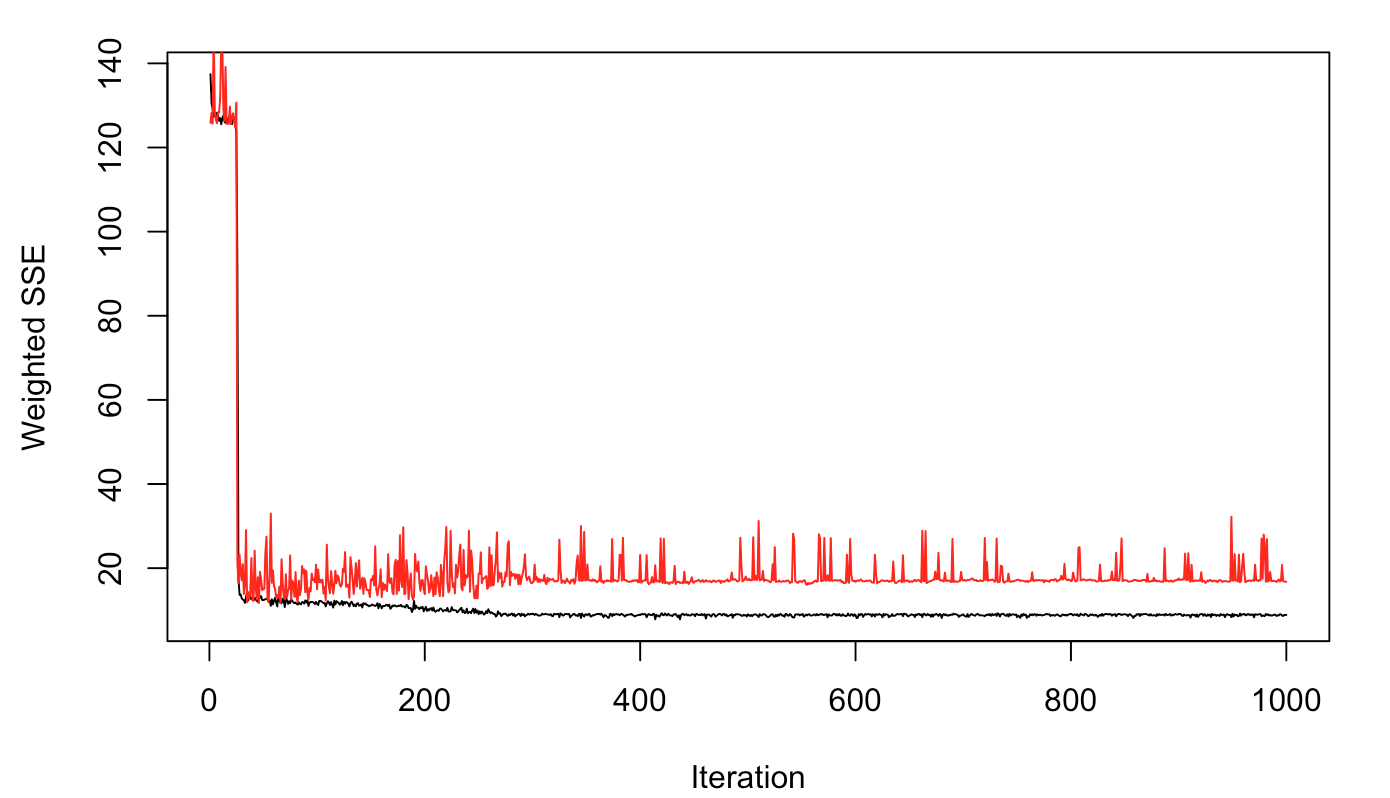
\includegraphics[scale=0.4]{imagens/9,8,8,5,3-1000.png}}
	\caption{Função de Custo 1000 iterações}
	\label{fig}
	\end{figure}
	
	\begin{table}[]
	\caption{Testes com limite de iterações}
	\begin{center}
    \begin{tabular}{l | c | r }
    \hline
         \# Iterações &Acurácia trenamento  & Acurácia teste \\\hline
         50 &97.42647  &95.65217    \\\hline
         100 &98.88268  &95.65217    \\\hline
         1000 &99.44341  &96.37681    \\\hline
         10000 &99.08088  &97.10145   \\\hline
         20000 &99.26471  &97.10145  \\\hline
    \end{tabular}
    \end{center}
    \end{table}
\section{Resultado e Discussão}

   
    
\section*{Conclusão}

  

\begin{thebibliography}{00}

\bibitem{b1} AN EVOLUTIONARY ARTIFICIAL NEURAL NETWORK APPROACH FOR BREAST CANCER DIAGNOSIS. Washington: Third International Conference on Knowledge Discovery and Data Mining, 2010. Anual. ISBN: 9781424463979.

\bibitem{b2} Livraria digital do Instituto de Engenheiros Eletricistas e Eletrônicos (IEEE), AN EVOLUTIONARY ARTIFICIAL NEURAL NETWORK APPROACH FOR BREAST CANCER DIAGNOSIS, disponível em https://ieeexplore.ieee.org/document/5432472, acesso em 20 de setembro de 2018.

\bibitem{b3} Pfizer, industria farmacêutica, O câncer de mama em números no Brasil e no mundo, disponível em https://www.pfizer.com.br/noticias/Cancer-de-mama-em-numeros, acesso em 15 de setembro de 2018.

\bibitem{b8} UCI Machine Learning Repository, Breast Cancer Wisconsin, disponível em http://archive.ics.uci.edu/ml/datasets/Breast+Cancer+Wisconsin+(Original), acesso em 25 de agosto de 2018.

\bibitem{b4} Salchenberger LM, Cinar E, Lash NA. Neural networks: A new tool for predicting thrift failures. Decision Sciences. 1992;23(4):899–916

\bibitem{b5} Ramchoun H, Amine M, Idrissi J, Ghanou Y, Ettaouil M. Multilayer Perceptron: Architecture Optimization and Training. International Journal of Interactive Multimedia and Artificial Intelligence. 2016;4(1):26–30.

\bibitem {b6} M. Ettaouil and Y. Ghanou, “Neural architectures optimization and Genetic algorithms”, Wseas Transactions On Computer, Issue 3, Volume 8, 2009, pp. 526-537. 

\bibitem {b7} T.B Ludermir “Hybrid Optimization Algorithm for the Definition of MLP Neural Network Architectures and Weights” Proceedings of the Fifth International Conference on Hybrid Intelligent Systems (HIS’05) 0-7695- 2457-5/05 20.00 2005 IEEE.

\bibitem{b9} Rosenblatt, “The Perceptron: A Theory of Statistical Separability in Cognitive Systems”, Cornell Aeronautical Laboratory, Report No. VG1196-G-1, January, 1958. 
\bibitem{b10} O. L. Mangasarian and W. H. Wolberg: "Cancer          diagnosis via linear 
      programming", SIAM News, Volume 23, Number 5, September 1990, pp 1 & 18.
\bibitem{b11} William H. Wolberg and O.L. Mangasarian: "Multisurface method of 
      pattern separation for medical diagnosis applied to breast cytology", 
      Proceedings of the National Academy of Sciences, U.S.A., Volume 87, 
      December 1990, pp 9193-9196.
\end{thebibliography}
\end{document}

